% !TeX root = ../main.tex
\chapter{Insiemi e operazioni}
\fonti{Lezioni 1, 2 e 3}

\section{Operazioni e appartenenza}
% A–L L1 pp. 1–2; M–Z L1. La logica resta proposizionale, senza funzioni caratteristiche.
Un insieme è determinato dai suoi elementi: $A=B$ significa che, per ogni $x$, $x\in A$ se e solo se $x\in B$. Equivalentemente si provano le due inclusioni $A\subseteq B$ e $B\subseteq A$. Si può descrivere un insieme per elenco, come $\{2,3,4\}$, oppure mediante una proprietà: $\Z=\{\ldots,-2,-1,0,1,2,\ldots\}$ e $\Q=\{a/b\mid a,b\in\Z,\ b\ne0\}$.

\begin{definizione}
Per due insiemi $A,B$ si definiscono
\[
\begin{aligned}
A\cup B&=\{x\mid x\in A\ \text{oppure}\ x\in B\},\\
A\cap B&=\{x\mid x\in A\ \text{e}\ x\in B\},\\
A\setminus B&=\{x\mid x\in A\ \text{e}\ x\notin B\},\\
A\triangle B&=(A\setminus B)\cup(B\setminus A).
\end{aligned}
\]
Sono, rispettivamente, \textbf{unione}, \textbf{intersezione}, \textbf{differenza} e \textbf{differenza simmetrica}. L'«oppure» dell'unione ammette che entrambe le appartenenze siano vere; nella differenza simmetrica ne deve essere vera esattamente una. Gli insiemi sono \textbf{disgiunti} se $A\cap B=\varnothing$.
\end{definizione}

\begin{schema}
\begin{tikzpicture}[scale=.67]
  \foreach \t/\lab in {0/Unione,4.5/Intersezione,9/Differenza,13.5/Diff. simmetrica}{
    \begin{scope}[shift={(\t,0)}]
      \ifdim\t pt=0pt\relax\fill[coloreschema!18] (0,0) circle (1);\fill[coloreschema!18] (1.2,0) circle (1);\fi
      \ifdim\t pt=4.5pt\relax\begin{scope}\clip (0,0) circle (1);\fill[coloreschema!18] (1.2,0) circle (1);\end{scope}\fi
      \ifdim\t pt=9pt\relax\begin{scope}\clip (0,0) circle (1);\fill[coloreschema!18] (-1,-1) rectangle (2.3,1);\fill[white] (1.2,0) circle (1);\end{scope}\fi
      \ifdim\t pt=13.5pt\relax\fill[coloreschema!18,even odd rule] (0,0) circle (1) (1.2,0) circle (1);\fi
      \draw (0,0) circle (1);\draw (1.2,0) circle (1);
      \node at (-.35,.5) {$A$};\node at (1.55,.5) {$B$};\node at (.6,-1.5) {\lab};
    \end{scope}
  }
\end{tikzpicture}
\end{schema}

\begin{proposizione}
Unione e intersezione sono commutative e associative:
\[
\begin{gathered}
A\cup B=B\cup A,\qquad A\cap B=B\cap A,\\
(A\cup B)\cup C=A\cup(B\cup C),\qquad
(A\cap B)\cap C=A\cap(B\cap C).
\end{gathered}
\]
Inoltre $A\triangle B=(A\cup B)\setminus(A\cap B)=B\triangle A$.
\end{proposizione}
\begin{proof}
Scambiare le due proposizioni «$x\in A$» e «$x\in B$» non cambia né la loro disgiunzione né la loro congiunzione: si ottiene la commutatività. Per l'associatività, entrambi i membri della prima identità richiedono che $x$ appartenga ad almeno uno tra $A,B,C$; entrambi i membri della seconda richiedono che appartenga a tutti e tre.

Infine, appartenere a uno solo fra $A$ e $B$ equivale ad appartenere alla loro unione, ma non alla loro intersezione. Anche questa condizione è invariata scambiando $A$ e $B$.
\end{proof}

\subsection{Unioni e intersezioni di famiglie}
\begin{definizione}
Sia $(A_i)_{i\in I}$ una famiglia di insiemi, con insieme degli indici $I$. Si pone
\[
\bigcup_{i\in I}A_i=\{x\mid \exists i\in I:\ x\in A_i\},\qquad
\bigcap_{i\in I}A_i=\{x\mid \forall i\in I:\ x\in A_i\}.
\]
Per l'intersezione si suppone $I\ne\varnothing$, oppure si fissa un ambiente $X$ e si limita la definizione agli $x\in X$. In quest'ultimo caso $\bigcap_{i\in\varnothing}A_i=X$; invece l'unione della famiglia vuota è sempre $\varnothing$.
\end{definizione}

% Integrazione M–Z L1 p. 2: proprietà dell'unione e dell'intersezione.
\begin{proposizione}
L'unione è il più piccolo insieme che contiene ogni $A_i$; l'intersezione è il più grande insieme contenuto in ogni $A_i$, nell'ambiente fissato.
\end{proposizione}
\begin{proof}
\textbf{Unione.} Ogni $x\in A_j$ appartiene all'unione scegliendo $i=j$, dunque $A_j\subseteq\bigcup_i A_i$. Se $A_i\subseteq B$ per ogni $i$, un elemento dell'unione sta in qualche $A_i$ e quindi in $B$: ne segue $\bigcup_i A_i\subseteq B$.

\textbf{Intersezione.} Ogni elemento dell'intersezione appartiene a ogni $A_j$. Se $B\subseteq A_i$ per ogni $i$, ciascun $x\in B$ appartiene a tutti gli $A_i$, dunque $B\subseteq\bigcap_i A_i$. Le convenzioni fissate danno le stesse proprietà anche per $I=\varnothing$.
\end{proof}

\begin{esercizio}[Associatività delle differenze]
Stabilire se la differenza e la differenza simmetrica sono associative.
\end{esercizio}
\begin{svolgimento}
\textbf{Differenza.} Per $A=B=C=\{0\}$ si ha $(A\setminus B)\setminus C=\varnothing$, mentre $A\setminus(B\setminus C)=\{0\}$. Quindi non è associativa. Non è neppure commutativa: $\{0\}\setminus\varnothing=\{0\}$ e $\varnothing\setminus\{0\}=\varnothing$.

\textbf{Differenza simmetrica.} Scomponiamo l'unione di tre insiemi secondo le appartenenze. Indichiamo con $A_0,B_0,C_0$ i punti appartenenti soltanto ad $A$, soltanto a $B$, soltanto a $C$; poniamo inoltre $T=A\cap B\cap C$. In formule,
\[
A_0=A\setminus(B\cup C),\quad B_0=B\setminus(A\cup C),\quad C_0=C\setminus(A\cup B).
\]
\passomath{(A\triangle B)\triangle C} I punti di $(A\triangle B)\setminus C$ stanno in uno solo fra $A,B$ e fuori da $C$: formano $A_0\cup B_0$. I punti di $C\setminus(A\triangle B)$ stanno in $C$ e, rispetto ad $A,B$, o in entrambi o in nessuno: formano $T\cup C_0$. Pertanto questo membro è $A_0\cup B_0\cup C_0\cup T$.

\passomath{A\triangle(B\triangle C)} I punti di $A\setminus(B\triangle C)$ stanno in $A$ e o in entrambi $B,C$ o in nessuno: formano $T\cup A_0$. I punti di $(B\triangle C)\setminus A$ formano $B_0\cup C_0$. Anche questo membro è dunque $A_0\cup B_0\cup C_0\cup T$. L'uguaglianza segue dall'associatività e dalla commutatività dell'unione.
\end{svolgimento}
% Ripresa effettiva A–L L3 pp. 1–2, confrontata con M–Z L2 pp. 5–6.

\begin{schema}
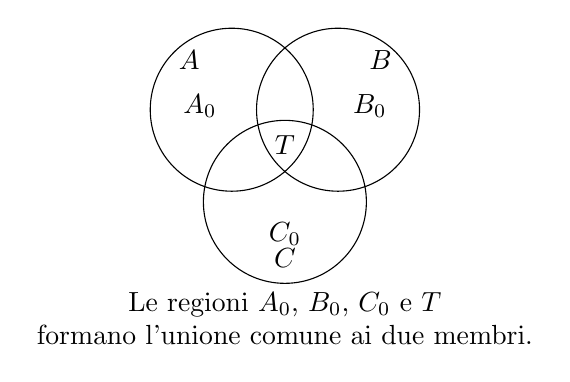
\begin{tikzpicture}[scale=.9]
  \draw (0,.45) circle (1.15);\draw (1.5,.45) circle (1.15);\draw (.75,-.85) circle (1.15);
  \node at (-.6,1.15) {$A$};\node at (2.1,1.15) {$B$};\node at (.75,-1.65) {$C$};
  \node at (-.45,.5) {$A_0$};\node at (1.95,.5) {$B_0$};\node at (.75,-1.3) {$C_0$};\node at (.75,-.05) {$T$};
  \node[align=center] at (.75,-2.5) {Le regioni $A_0$, $B_0$, $C_0$ e $T$\\formano l'unione comune ai due membri.};
\end{tikzpicture}
\end{schema}

\section{Prodotti cartesiani}
% A–L L1 pp. 3–4. Le potenze con insieme di indici sono rinviate alle funzioni.
\begin{definizione}
Il \textbf{prodotto cartesiano} è $A\times B=\{(a,b)\mid a\in A,\ b\in B\}$. Le coppie sono ordinate: $(a,b)=(a',b')$ se e solo se $a=a'$ e $b=b'$. Più in generale,
\[
A_1\times\cdots\times A_n=\{(a_1,\ldots,a_n)\mid a_i\in A_i\text{ per }i=1,\ldots,n\}.
\]
Se i fattori sono tutti $A$, si scrive $A^n$. In particolare $\R^2=\R\times\R$ è il piano delle coppie di numeri reali.
\end{definizione}

\begin{esempio}
Se $A=\{m,n,p\}$ e $B=\{9,8\}$, allora
\[
A\times B=\{(m,9),(m,8),(n,9),(n,8),(p,9),(p,8)\}.
\]
Il prodotto è vuoto se un fattore è vuoto; se entrambi sono non vuoti, scegliendo un elemento in ciascuno si ottiene una coppia nel prodotto. In generale $A\times B\ne B\times A$: scambiare le coordinate cambia le coppie, pur dando una corrispondenza uno a uno tra i due prodotti.
\end{esempio}

\section{Parti, complementi e identità}
% A–L L2 pp. 1–2; integrazioni logiche M–Z L2 pp. 2–6 e L3 p. 1.
\begin{definizione}
L'\textbf{insieme delle parti} di $X$ è $\mathcal P(X)=\{A\mid A\subseteq X\}$. Per $A\subseteq X$, il \textbf{complementare} nell'ambiente $X$ è $A^c=X\setminus A$, indicato anche con $C(A)$.
\end{definizione}

\begin{esempio}
Per $X=\{2,3,4\}$,
\[
\mathcal P(X)=\{\varnothing,\{2\},\{3\},\{4\},\{2,3\},\{2,4\},\{3,4\},X\}.
\]
Si distingue $A\subseteq X$ da $A\in\mathcal P(X)$: dicono la stessa cosa, ma la seconda considera $A$ come un elemento di un nuovo insieme.
\end{esempio}

\begin{schema}
\begin{tikzpicture}[scale=.75]
  \fill[coloreschema!16] (0,0) rectangle (4.5,2.4);\fill[white] (1.5,1.2) circle (.8);
  \draw (0,0) rectangle (4.5,2.4);\draw (1.5,1.2) circle (.8);
  \node at (1.5,1.2) {$A$};\node at (3.3,1.2) {$A^c$};\node[above right] at (4.5,2.2) {$X$};
\end{tikzpicture}
\end{schema}

\subsection{Logica delle appartenenze}
Fissato $x$, poniamo $\alpha=(x\in A)$ e $\beta=(x\in B)$. Le operazioni corrispondono ai connettivi logici secondo la tabella seguente; $\neg$ denota la negazione, $\lor$ l'«oppure» e $\land$ l'«e».
\[
\begin{array}{cc|cccc}
\alpha&\beta&x\in A\cup B&x\in A\cap B&x\in A\setminus B&x\in A\triangle B\\\hline
\mathrm V&\mathrm V&\mathrm V&\mathrm V&\mathrm F&\mathrm F\\
\mathrm V&\mathrm F&\mathrm V&\mathrm F&\mathrm V&\mathrm V\\
\mathrm F&\mathrm V&\mathrm V&\mathrm F&\mathrm F&\mathrm V\\
\mathrm F&\mathrm F&\mathrm F&\mathrm F&\mathrm F&\mathrm F
\end{array}
\]
Un'implicazione $\alpha\Rightarrow\beta$ è falsa soltanto quando $\alpha$ è vera e $\beta$ è falsa. Si verifica quindi, riga per riga, che
\[
(\alpha\Rightarrow\beta)\iff(\neg\alpha\lor\beta),\qquad
\neg(\alpha\Rightarrow\beta)\iff(\alpha\land\neg\beta).
\]
L'inclusione è un'affermazione universale: $A\subseteq B$ equivale a $\forall x\,(x\in A\Rightarrow x\in B)$. La sua negazione è $\exists x\,(x\in A\land x\notin B)$: un solo controesempio basta a negarla.

\begin{esercizio}[Negazione di un'implicazione]
La negazione di $\alpha\Rightarrow\beta$ coincide con un'implicazione il cui antecedente e conseguente siano scelti tra $\alpha,\beta,\neg\alpha,\neg\beta$?
\end{esercizio}
\begin{svolgimento}
La negazione cercata è vera in una sola delle quattro combinazioni di verità. Invece ogni implicazione del tipo indicato è vera almeno nelle due combinazioni in cui il suo antecedente è falso. Non possono quindi coincidere. La restrizione sulle formule ammesse è essenziale per la domanda.
\end{svolgimento}

\begin{esercizio}[Complementazione e leggi di De Morgan]
Verificare $(A^c)^c=A$ e dimostrare $(A\cup B)^c=A^c\cap B^c$, $(A\cap B)^c=A^c\cup B^c$.
\end{esercizio}
\begin{svolgimento}
Tutte le appartenenze sono considerate per $x\in X$. Non appartenere al complementare di $A$ equivale ad appartenere ad $A$, quindi $(A^c)^c=A$.

\passomath{(A\cup B)^c=A^c\cap B^c} Non appartenere all'unione significa non appartenere né ad $A$ né a $B$: $\neg(\alpha\lor\beta)\iff\neg\alpha\land\neg\beta$.

\passomath{(A\cap B)^c=A^c\cup B^c} Non appartenere all'intersezione significa che almeno una delle due appartenenze è falsa: $\neg(\alpha\land\beta)\iff\neg\alpha\lor\neg\beta$. Le equivalenze si possono anche controllare nelle quattro righe della tabella.
\end{svolgimento}

\begin{proposizione}[Distributività]
Per insiemi $A,B,C$ valgono
\[
\begin{aligned}
(A\cup B)\cap C&=(A\cap C)\cup(B\cap C),\\
(A\cap B)\cup C&=(A\cup C)\cap(B\cup C),\\
(A\triangle B)\cap C&=(A\cap C)\triangle(B\cap C).
\end{aligned}
\]
\end{proposizione}
\begin{proof}
Per la prima, $x$ deve appartenere a $C$ e ad almeno uno tra $A,B$: questo equivale a stare in $A\cap C$ oppure in $B\cap C$.

Per la seconda, se $x\in C$, appartiene a entrambi i membri. Se $x\notin C$, il primo richiede $x\in A\cap B$, e il secondo richiede simultaneamente $x\in A$ e $x\in B$: ancora la stessa condizione.

Per la terza, se $x\notin C$, non sta in nessuno dei due membri. Se $x\in C$, in entrambi i membri si richiede che stia in uno solo fra $A$ e $B$. I casi esauriscono le possibilità.
\end{proof}

\begin{esercizio}[Elementi neutri e annullamento]
In $\mathcal P(X)$ verificare $A\triangle\varnothing=A$ e $A\cap X=A$. Dato $A$, esiste $B$ tale che $A\triangle B=\varnothing$? Per quali $A$ esiste $B$ tale che $A\cap B=X$?
\end{esercizio}
\begin{svolgimento}
La differenza simmetrica con $\varnothing$ conserva esattamente gli elementi di $A$; l'intersezione con $X$ conserva tutti gli elementi di $A\subseteq X$. Questi sono gli elementi neutri per le due operazioni.

L'uguaglianza $A\triangle B=\varnothing$ dice che nessun elemento appartiene a uno solo tra $A,B$, cioè $A=B$. Quindi $B=A$ è sempre l'unica soluzione.

Se $A\cap B=X$, allora $X\subseteq A\subseteq X$ e $X\subseteq B\subseteq X$, dunque $A=B=X$. Viceversa questa scelta dà l'uguaglianza. Solo l'elemento $A=X$ ammette una soluzione per la seconda richiesta.
\end{svolgimento}
